% ========================================
% Some basic settings
% ========================================
\documentclass[a4paper]{article}

\usepackage[left=1.5cm,right=1.5cm,bottom=2cm,top=2cm]{geometry}
\usepackage[ngerman,shorthands=off]{babel}
\usepackage{xcolor}
\usepackage{hyperref}
\hypersetup{
    colorlinks,
    allcolors=blue
}

\title{Klausurfragen vom 03.02.2025}
\author{\href{https://github.com/minus-n/BiWi-Klausurzusammenfassung}{github/minus-n}}

\usepackage[default]{sourcesanspro}
\usepackage[T1]{fontenc}

% ========================================
% Primary definitions (not intended for direct use)
% ========================================

\usepackage{xfp}

%% thank you, internet
\usepackage{enumitem}
\usepackage{amssymb}
\usepackage{pifont}
\usepackage{wasysym}
\usepackage{graphicx}
\usepackage{tcolorbox}

% helpers for multiple choice questions
\newcommand{\ACorrectAnswer}{\rlap{$\square$}{\raisebox{2pt}{\large\hspace{1pt}\ding{51}}}\hspace{-2.5pt}}
\newcommand{\AWrongAnswer}{\rlap{$\square$}{\large\hspace{1pt}\ding{55}}}
\newcommand{\AnUnsureAnswer}{\rlap{$\square$}{\large\hspace{1pt}\textbf?}}
\newlist{multiple-choice-list}{itemize}{2}
\setlist[multiple-choice-list]{label=$\square$}

% helpers for single-choice questions
\newlist{single-choice-list}{itemize}{2}
\setlist[single-choice-list]{label=$\ocircle$}
\newcommand{\TheCorrectAnswer}{\rlap{\hspace{1.4pt}$\bullet$}{$\ocircle$}}
\newcommand{\TheWrongAnswer}{$\ocircle$}
\newcommand{\TheUnsureAnswer}{\rlap{\hspace{1.4pt}\textbf?}{$\ocircle$}}
% thank you, internet

% helpers for mapping questions
\newtcolorbox{mapping-box}{colback=black!5,colframe=black!75,sidebyside}

\newcommand{\defaultCorrect}{\ding{51}}
\newcommand{\defaultWrong}{\ding{55}}
\newcommand{\defaultUnsure}{\textbf{?}}


% ========================================
% Secondary definition (intended for use in the document)
% ========================================


% those definitions will change
\newenvironment{answers}{\begin{itemize}}{\end{itemize}}

\newcommand{\correct}{\defaultCorrect}
\newcommand{\wrong}{\defaultWrong}
\newcommand{\unsure}{\defaultUnsure}

\setcounter{secnumdepth}{0}
\newenvironment{question}[2]{%
    \section[#1 \normalfont(#2)]{#1\\\small\normalfont\hyperlink{tableofcontents}{zurück zum Inhaltsverzeichnis}}%
}{%
    \newpage%
}

\newcommand{\questiontext}[1]{\textbf{#1}}
\newcommand{\assignment}[1]{\textbf{\textit{#1}}\newline}


\newenvironment{multiple-choice}[1]{%
    \begin{question}{#1}{Multiple Choice}%
    \renewenvironment{answers}{%
        \begin{multiple-choice-list}}{\end{multiple-choice-list}%
    }%
    \renewcommand{\correct}{\ACorrectAnswer}%
    \renewcommand{\wrong}{\AWrongAnswer}%
    \renewcommand{\unsure}{\AnUnsureAnswer}%
}%
{%
    \renewcommand{\correct}{\defaultCorrect}%
    \renewcommand{\wrong}{\defaultWrong}%
    \renewcommand{\unsure}{\defaultUnsure}%
    \end{question}%
}

\newenvironment{single-choice}[1]{%
    \begin{question}{#1}{Single Choice}%
    \renewenvironment{answers}{%
        \begin{single-choice-list}}{\end{single-choice-list}%
    }%
    \renewcommand{\correct}{\TheCorrectAnswer}%
    \renewcommand{\wrong}{\TheWrongAnswer}%
    \renewcommand{\unsure}{TheUnsureAnswer}%
}{%
    \renewcommand{\correct}{\defaultCorrect}%
    \renewcommand{\wrong}{\defaultWrong}%
    \renewcommand{\unsure}{\defaultUnsure}%
    \end{question}%
}

\newenvironment{mapping}[1]{%
    \begin{question}{#1}{Zuordnungsaufgabe}%
    \newcommand{\ismappedto}{\tcblower}%
    \newenvironment{answer}{\begin{mapping-box}}{\end{mapping-box}}%
}{%
    \end{question}%
}

% ========================================
% The actual document
% ========================================

\begin{document}

% ========================================
% Title and Table of Contents
% ========================================

\maketitle
\newpage
\hypertarget{tableofcontents}{}
\tableofcontents
\newpage

% ========================================
% Questions and Answers
% ========================================

\begin{multiple-choice}{Fragen im Lehr-/Lernkontext}
    \assignment{Bitte kreuzen Sie die richtige(n) Aussage(n) an!}
    \questiontext{In Bezug auf Fragen der Lehrkraft an Schüler*innen gilt:}
    \begin{answers}
        \item[\correct] Wissensfragen dienen im Lernprozess dem Üben des Abrufs von Fakten, Begriffen und Handlungen.
        \item[\correct] Sie dienen im Fragen-entwickelnden Unterricht oft der Steuerung des Unterrichtsgesprächs.
        \item[\wrong] Denkfragen können im Besonderen der Ebene des Erinnerns in der Taxonomie der Wissensnutzung nach Bloom zugeordnet werden.
        \item[\wrong] Bei der Frage „Hätte Kolumbus seine Fahrt auch unternommen, wenn er geglaubt hätte, dass die Erde eine Scheibe ist?” geht es primär um die Ebene des Anwendens nach Bloom (= Ausführen von Handlungen).
    \end{answers}
\end{multiple-choice}

\begin{single-choice}{Prinzipien effektiver Klassenführung III}
    \assignment{Trifft folgende Aussage zu?}
    \questiontext{Die Ankündigung einer Aufgabe mit den Worten „Jetzt wollen wir mal sehen, wer von euch ...“ ist eine Verhaltensweise seitens der Lehrkraft, mit der die Gruppenmobilisierung gefördert wird.}
    \begin{answers}
        \item[\correct] trifft nicht zu
        \item[\wrong] trifft zu
    \end{answers}
\end{single-choice}

\begin{single-choice}{Lernen als aktive Wissenskonstruktion}
    \assignment{Trifft folgende Aussage zu?}
    \questiontext{Empirische Befunde deuten darauf hin, dass ein unterstützendes Unterrichtsklima - über eine höhere Lernmotivation und ein stärkeres Engagement der Schüler*innen - einen eher indirekten Effekt auf den Lernerfolg hat.}
    \begin{answers}
        \item[\correct] trifft zu
        \item[\wrong] trifft nicht zu 
    \end{answers}
\end{single-choice}

\begin{mapping}{Lernen als aktive Wissenskonstruktion}
    \assignment{Es gibt gemäß Mayer (1996) drei grundlegende kognitive Prozesse, die an der Konstruktion von Wissen beteiligt sind, nämlich Auswahl, Organisation und Integration. Ordnen sie die Tätigkeitsbereiche jeweils dem entsprechenden kognitiven Prozess zu.}
    \begin{answer}
        Auswählen
        \ismappedto
        Ein Schüler entscheidet sich beim Lesen eines Lehrbuchtextes dafür, ausschließlich die Passagen die er zuvor markiert hat, zu lernen.
    \end{answer}
    \begin{answer}
        Organisation
        \ismappedto
        Eine Schülerin bringt beim Lernen Informationen in eine Ursache-Wirkungsbeziehung.
    \end{answer}
    \begin{answer}
        Integration
        \ismappedto
        Beim Lernen überlegt sich ein Schüler für die neu erhaltenen Informationen Beispiele aus seinem Alltag.
    \end{answer}
\end{mapping}

\begin{multiple-choice}{Cognitive Load Theory}
    \assignment{Bitte kreuzen sie die beiden richtigen Aussagen an!}
    \questiontext{Nach der Cognitive Load Theory...}
    \begin{answers}
        \item[\correct] ist die intrinsische Belastung hoch, wenn Schüler*innen beim Erstellen einer Präsentation mit PowerPoint aufgrund ihrer mangelnden Erfahrung der Bedienung des Programms mehr Aufmerksamkeit widmen als dem Durcharbeiten des zu präsentierenden Stoffes.
        \item[\correct] sollte die Physiklehrerin nach den Prinzip der zeitlichen Kontiguität wichtige Handlungen und Ereignisse erläutern, \underline{während} (anstatt bevor) sie den Schüler*innen ein Experiment vorführt.
        \item[\wrong] kann die extrinsische Belastung, also die von den Schüler*innen wahrgenommene Komplexität des Lernstoffs, unabhängig vom Vorwissen der Schüler*innen bestimmt werden.
        \item[\wrong] kann die Lehrkraft die intrinsische Belastung der Schüler*innen nicht beeinflussen, ohne die Lernziele zu ändern.
    \end{answers}
\end{multiple-choice}

\begin{mapping}{Selbstbestimmungstheorie der Motivation (Deci \& Ryan, 2000)}
    \assignment{Bitte ordnen Sie die Beispiele bezüglich des Anreizes, der zum Lernen führt, der jeweils passenden Regulationsform zu.}
    \begin{answer}
        Integrierte Regulation
        \ismappedto
        Die Schülerin lernt Mathematik, da sie sonst ein schlechtes Gewissen hätte.
    \end{answer}
    \begin{answer}
        Introjizierte Regulation
        \ismappedto
        Die Schülerin lernt Mathematik, weil sie sich selbst als mathematisch begabte Person ansieht.
    \end{answer}
    \begin{answer}
        Internale Regulation
        \ismappedto
        Der Schüler lernt Mathematik, da es ihm Freude bereitet.
    \end{answer}
    \begin{answer}
        Externale Regulation
        \ismappedto
        Der Schüler lernt Mathematik, da er dann ein Lob von seinen Eltern bekommt.
    \end{answer}
    \begin{answer}
        Identifizierte Regulation
        \ismappedto
        Die Schülerin lernt Mathematik, weil sie gut in diesem Fach sein möchte.
    \end{answer}
\end{mapping}

\begin{multiple-choice}{Prävention \& Intervention bei Unterrichtsstörungen}
    \assignment{Bitte kreuzen Sie die richtige(n) Aussage(n) an!}
    \questiontext{In Hinblick auf die Prävention und Intervention bei Unterrichtsstörungen gelten folgende Aussagen:}
    \begin{answers}
        \item[\correct] Anreize für die Klasse können leicht mittels Tokens und durch Berücksichtigung des Premack-Prinzips realisiert werden.
        \item[\correct] Wenn man eine Schülerin, die häufig stört, ständig ermahnt, und dabei vergisst, positives Verhalten zu verstärken, kann diese Reaktionsweise der Lehrkraft dazu führen, dass eine „Negativspirale“ entsteht und das störende Verhalten immer stärker zunimmt.
        \item[\correct] In Anbetracht der Vorgaben zur Prävention durch Präsenz- und Stoppsignale gemäß Nolting (2007) ist es wichtig, dass die Lehrkraft auch flüchtige Vorgänge, die eine Unterrichtsstörung darstellen, keinesfalls ignoriert.
        \item[\wrong] Durch Bestrafung können SuS dabei unterstützt werden, ein alternatives und angemessenes Verhalten aufzubauen.
    \end{answers}
\end{multiple-choice}

\begin{multiple-choice}{Operantes Konditionieren}
    \assignment{Bitte kreuzen Sie die richtige(n) Aussage(n) an!}
    \questiontext{Bewerten Sie die folgenden Aussagen und Fälle zum operanten Konditionieren}
    \begin{answers}
        \item[\unsure] Wenn ein Schüler seine Angst vor Klassenarbeiten dadurch zu reduzieren versucht, dass er bei Klassenarbeiten wegen Krankheit fehlt, wirkt die Reduktion der Angst als negativer Verstärker seines Fehlens bei Klassenarbeiten.
        \item[\correct] Token-Ökonomien sind Verstärkungspläne, bei denen primäre Verstärker (z.B. Bonbons, Kekse, Erfrischungsgetränke) eine Verhaltensformung durch die Kombination von Belohnungen und Bestrafungen ermöglichen.
        \item[\correct] Wenn ich als Lehrkraft 10 grüne Flasche an die Tafel male, wobei jede Flasche 5 Minuten Spielzeit symbolisiert und bei jedem Verstoß in der Klasse gegen die Ruheregel eine Flasche durchstreiche, dann ist das als positive Bestrafung zu sehen.
        \item[\wrong] Auf das immer stärker werdende Quengeln seiner Tochter an der Supermarktkasse reagiert der Vater damit, dass er ihr die ersehnten Marshmallows kauft, worauf die Tochter das Quengeln einstellt. Aus operanter Sicht verstärkt sich der Vater selbst mit seinem Verhalten negativ.
    \end{answers}
\end{multiple-choice}

\begin{multiple-choice}{Motivation \& Emotion}
    \assignment{Bitte kreuzen Sie diejenige Aussage an, die richtig ist!}
    \questiontext{In Hinblick auf die Motivation bzw. die Emotion gilt:}
    \begin{answers}
        \item[\correct] Dass von einer introjizierten Regulation gesprochen werden kann, wenn ein Schüler etwas tut, weil er den Erwartungen seiner Eltern gerecht werden möchte und weil er sonst ein schlechtes Gewissen bekäme.
        \item[\wrong] Mit dem Begriff Stimmung werden Gefühlsregungen umschrieben, die relativ konkret bestimmbar sind und sich meist auf einen Auslöser zurückführen lassen.
        \item[\wrong] Extrinsisch motivierte Verhaltensweisen können durch die Prozesse der Internalisation und Integration nicht in selbstbestimmte Handlungen überführt werden.
        \item[\wrong] Die Selbstbestimmungstheorie geht von der anthropologischen Grundannahme aus, dass Menschen bereit sind, Wertmaßstäbe der Gesellschaft zu internalisieren, weil sie sich so eine Maxmierung des persönlichen Nutzens für sich erhoffen. 
    \end{answers}
\end{multiple-choice}

\begin{single-choice}{Prinzipien effektiver Klassenführung II}
    \assignment{Trifft folgende Aussage zu?}
    \questiontext{Im Beispiel „Nach Übungen im Rechtschreiben sollen die Rechtschreibsachen weggelegt werden und die Rechenbücher hervorgeholt werden. Als fast alle Rechenbücher auf dem Tisch liegen, kommt die Lehrkraft auf die Rechtschreibübungen zurück und fragt: ‚Wer von euch hat alle Wörter richtig geschrieben?\relax‘“ werden die Momente Reibungslosigkeit und Schwung gelungen umgesetzt.}
    \begin{answers}
        \item[\correct] trifft nicht zu
        \item[\wrong] trifft zu
    \end{answers}
\end{single-choice}

\begin{mapping}{Emotional Support}
    \questiontext{Lesen sie die vier folgenden Unterrichtsszenarien durch und ordnen Sie jedes Szenario der passenden Subdimension (Positive Climate, Negative Climate, Teacher Sensitivity, Regard for Adolescent Perspectives) des Bereichs Emotional Support (Hafen et al., 2014) zu.}
    \begin{answer}
        Negative Climate
        \ismappedto
        Während einer Gruppenarbeit herrscht eine spürbar angespannte Stimmung. Die Lehrkraft reagiert mit sichtbarer Ungeduld, wenn Schüler*innen Fragen haben oder Fehler machen. Einmal kommentiert sie vor der ganzen Klasse: „Das hättest du dir aber wirklich denken können!“, woraufhin einige Schüler*innen leise kichern, ohne dass eingegriffen wird.
    \end{answer}
    \begin{answer}
        Teacher Sensitivity
        \ismappedto
        Nach dem Unterricht bittet die Lehrkraft eine Schülerin, die in letzter Zeit still war, kurz zum Gespräch. Dabei erkundigt sie sich, ob es möglicherweise schulische oder außerschulische Gründe gibt, weshalb sie kaum noch mitarbeitet.
    \end{answer}
    \begin{answer}
        Regard for Adolescent Perspectives
        \ismappedto
        Zu Beginn einer neuen Unterrichtseinheit gibt die Lehrkraft mehrere mögliche Projektthemen vor, die für die Klasse interessant sein könnten. Sie lässt die Schüler*innen in Kleingruppen über die Themen diskutieren und stimmt anschließend gemeinsam über die Schwerpunkte ab. Die Gruppen dürfen anschließend entscheiden, wie sie ihre Projektergebnisse präsentieren wollen, etwa in Form von Videos, Podcasts oder Postern.
    \end{answer}
    \begin{answer}
        Positive Climate
        \ismappedto
        In einem Klassenkreis zum Thema „Zusammenarbeit und Respekt“ lässt die Lehrkraft die Schüler*innen offen im Plenum darüber sprechen, welche Regeln und Umgangsformen ihnen wichtig sind. Sie steuert wenig direkt, achtet jedoch darauf, dass alle sich gegenseitig zuhören und ermutigt freundliche, sich z.B. bei unsicheren Beiträgen konkret zu äußern, was den Schüler*innen hilft, ihre Standpunkte zu vertreten.
    \end{answer}
\end{mapping}

\begin{mapping}{Erziehnugsstile nach Baumrind}
    \questiontext{Lesen Sie sich die folgenden vier Fallbeispiele zu elterlichem Verhalten durch und ordnen Sie jedem Beispiel den entsprechenden Erziehungsstil nach Baumrind (1991) zu.}
    \begin{answer}
        Ein Vater legt fest, dass seine zehnjährige Tochter jeden Abend um 20Uhr im Bett sein soll. Sie bittet allerdings darum, abends noch ein Buch lesen zu dürfen. Der Vater erklärt ihr in Ruhe, warum ein geregelter Schlaf wichtig ist, hört sich ihre Argumente an und kommt ihr entgegen, indem er die Schlafenszeit um 15 Minuten verschiebt. Er macht aber auch deutlich, dass dies nur funktioniert, wenn sich sich morgens rechtzeitig fertig macht und nicht müde in die Schule geht.
        \ismappedto
        Autoritativer Erziehungsstil
    \end{answer}
    \begin{answer}
        Eine Mutter besteht darauf, dass ihr achtjähriger Sohn jeden Abend um Punkt 19 Uhr im Bett zu liegen hat. Wenn er widerspricht oder noch nicht müde ist, reagiert sie mit Strenge und sagt: „Du gehst jetzt sofort ins Bett, weil ich das so sage, und darüber wird nicht diskutiert!“ Sollte er nicht gehorchen, drohen Strafen wie Fernseh- oder Handyverbot.
        \ismappedto
        Autoritärer Erziehungsstil
    \end{answer}
    \begin{answer}
        Ein neunjähriger Junge darf abends so lange fernsehen, wie er möchte. Seine Eltern legen keine festen Zeiten fest, weil sie ihm „seinen Freiraum“ lassen wollen. Wenn er einmal bis Mitternacht aufbleibt und am nächsten Tag unausgeschlafen in die Schule geht, erhalten die Entscheidungen keinerlei Konsequenzen. Hauptsache, das Kind fühlt sich wohl.
        \ismappedto
        Pessimistischer Erziehungsstil
    \end{answer}
    \begin{answer}
        Eine zwölfjährige Tochter verbringt ihre Abende häufig allen und darf unbegrenzt an Computer oder Smartphone bleiben. Die Eltern interessieren sich kaum noch dafür, wie lange sie wach ist oder was sie macht. Auch wenn das Mädchen häufiger Probleme in der Schule hat, reagieren sie nur selten oder zeigen Desinteresse.
        \ismappedto
        Vernachlässigter Erziehungsstil
    \end{answer}
\end{mapping}

\begin{mapping}{Operante Konditionierung - Verstärkerpläne}
    \assignment{Ordnen Sie die Beispiele dem jeweils passenden Verstärkerplan zu.}
    \begin{answer}
        Variabler Quotenplan
        \ismappedto
        „Wenn ihr genügend Aufgaben gelöst habt, gibt es eine Klassenbelohnung.“
    \end{answer}
    \begin{answer}
        Variabler Intervallplan
        \ismappedto
        „Ich komme später wieder bei euch vorbei. Wer dann konzentriert arbeitet, kann sich einen Hausaufgabengutschein abholen.“
    \end{answer}
    \begin{answer}
        Kontinuierliche Verstärkung
        \ismappedto
        „Für jede richtige Wortmeldung gibt es heute einen Smiley-Aufkleber.“
    \end{answer}
    \begin{answer}
        Fester Quotenplan
        \ismappedto
        „Wer von euch für zehn englische Vokabeln den passenden deutschen Begriff nennen kann, muss heute keine Hausaufgaben machen.“
    \end{answer}
    \begin{answer}
        Fester Intervallplan
        \ismappedto
        „Ich komme in 30 Minuten zurück und wer dann fleißig arbeitet, darf schon in die Pause gehen.“
    \end{answer}
\end{mapping}

\begin{multiple-choice}{Drei-Speicher-Modell}
    \assignment{Biite kreuzen Sie die richtige(n) Aussage(n) an!}
    \questiontext{Beim Drei-Speicher-Modell des Gedächtnisses gilt:}
    \begin{answers}
        \item[\correct] Dass im Langzeitgedächtnis das Wissen in Form verbal-semantischer sowie bildhaft-analoger Repräsentationen gespeichert ist.
        \item[\correct] Dass intentionales Auswählen im Arbeitsgedächtnis stattfindet, während spontanes Auswählen im sensorischen Speicher stattfindet.
        \item[\wrong] Dass auch das Langzeitgedächtnis, ähnlich wie das Arbeitsgedächtnis, nur eine begrenzte Menge an Informationen aufnehmen kann.
        \item[\wrong] Dass beim Cocktail-Party-Phänomen deutlich wird, dass das persönliche Vorwissen nicht schon für die Auswahl an Daten im sensorischen Speicher relevant ist.
    \end{answers}
\end{multiple-choice}

\begin{multiple-choice}{Arbeits- oder Kurzzeitgedächtnis}
    \assignment{Bitte kreuzen Sie die richtige(n) Aussage(n) an!}
    \questiontext{Im Arbeits- oder Kurzzeitgedächtnis}
    \begin{answers}
        \item[\correct] werden Schemata aus dem Langzeitgedächtnis herangezogen, um Informationen zu größeren, umfassenden Einheiten zusammenzufassen (Chunking).
        \item[\correct] wird die Größe der Chunks, die gebildet werden können, durch das Vorwissen bestimmt.
        \item[\wrong] werden Inhalte bereits nach wenigen Tagen wieder vergessen, sofern sie nicht im Langzeitgedächtnis dauerhaft gespeichert werden.
        \item[\wrong] werden räumlich-visuelle Informationen im Phonological Loop (phonologische Schleife) verarbeitet.
    \end{answers}
\end{multiple-choice}

\begin{multiple-choice}{Kooperatives Lernen II}
    \assignment{Bitte kreuzen Sie die richtige(n) Aussage(n) an!}
    \questiontext{Beim kooperativen Lernen gelten folgende Aussagen:}
    \begin{answers}
        \item[\correct] Die Wirksamkeit von Reciprocal Teaching lässt sich damit erklären, dass die Schüler*innen ein verändertes Modell über die Aufgabe des Lesens entwickeln und Lesen in zunehmenden Maße als eine konstruktive Aktivität begreifen, die eine aktive Auseinandersetzung mit dem Text fordert.
        \item[\correct] Dass beim Gruppenpuzzle den Expertengruppen eine sozial-integrative Funktion zukommt, weil dort schwächere Schüler*innen mithilfe der Leistungsstärken auch zu Expert*innen für ein Thema werden können.
        \item[\wrong] Gemäß der neo-piagetschen Perspektive wird der Interaktion mit Peers ein höheres lernförderliches Potential eingeräumt als der Interaktion mit Weiterentwickelten (z.B. Lehrkräften).
        \item[\wrong] Dass nach der neo-vygotskyschen Perspektive ein kognitives Modellieren und Internalisieren von Lernprozessen im Rahmen kooperativer Lernarrangements nicht realisierbar ist. 
    \end{answers}
\end{multiple-choice}

\begin{multiple-choice}{Lernziele II}
    \assignment{Bitte kreuzen Sie das/die richtig formulierte(n) Lernziel(e) an!}
    \questiontext{Welches/welche der nachfolgenden Lernziele ist/sind gemäß Wittwer et al. (2019) richtig formuliert?}
    \begin{answers}
        \item[\correct] Schüler*innen kennen die einzelnen Phasen der Meiose.
        \item[\correct] Schüler*innen können das Plusquamperfekt von Verben im Englischen bilden.
        \item[\wrong] Die Schüler*innen können schwierige Texte lesen.
        \item[\wrong] Die Schülerinnen und Schüler schauen einen Film zum Sonnensystem.   
    \end{answers}
\end{multiple-choice}

\begin{multiple-choice}{Gestaltung von Erklärungen}
    \assignment{Bitte kreuzen Sie die beiden Aussagen an!}
    \questiontext{Bei der sprachlichen Gestaltung von Erklärungen gilt:}
    \begin{answers}
        \item[\correct] Dass benachbarte Sätze durch gemeinsame bzw. überlappende Argumente beim Lesen oder Hören leichter miteinander verbunden und verstanden werden können.
        \item[\correct] Dass man nach der Richtlinie der Prinzipienorientierung bei prozeduralen Erklärungen erläutert, warum ein bestimmter Lösungsschritt sinnvoll ist und wozu er dient.
        \item[\wrong] Dass kohäsive Erklärungen von Lernenden als weniger verständlich beurteilt werden als nicht-kohäsive Erklärungen.
        \item[\wrong] Dass eine Adaption an das Vorwissen der Lernenden am besten gelingt, wenn man einheitlich allen Lernenden möglichst einfache und anschauliche Erklärungen gibt.
    \end{answers}
\end{multiple-choice}

\begin{multiple-choice}{Repräsentation von Wissen}
    \assignment{Bitte kreuzen Sie die richtige(n) Aussage(n) an!}
    \questiontext{In Bezug auch die Repräsentation von Wissen im Langzeitgedächtnis gelten folgende Aussagen:}
    \begin{answers}
        \item[\correct] Schemata sind abstrakte Wissenstrukturen, die das Einordnen und Erkennen von Gegenständen in der Welt ermöglichen.
        \item[\correct] Wissenserwerb kann als die Konstruktion und Ausdifferenzierung von Schemata verstanden werden.
        \item[\unsure] Beim Lesen von Sätzen merken sich Menschen intuitiv den genauen Wortlaut.
        \item[\wrong] Das Wissen darüber, was Sie selbst an Silvester 2019 gemacht haben, lässt sich als semantisches Wissen bezeichnen.
    \end{answers}
\end{multiple-choice}

\begin{multiple-choice}{Lernen}
    \assignment{Bitte kreuzen Sie die richtige(n) Aussage(n) an!}
    \questiontext{In Bezug auch Lernen gilt Folgendes:}
    \begin{answers}
        \item[\correct] Lernen ist definiert als die Fähigkeit, regelhaft und adaptiv auf sich ändernde Umweltbedingungen zu reagieren.
        \item[\wrong] Auch temporäre Veränderungen im Individuum wie Stimmungsschwankungen oder Bewusstseinstrübungen können als Lernen aufgefasst werden.
        \item[\wrong] Lernen ist auch ohne Gedächtnis möglich.
        \item[\wrong] Reifungsprozesse im Gehirn können die Fähigkeit, zu lernen, erheblich einschränken.
    \end{answers}
\end{multiple-choice}

\begin{mapping}{Hauptprobleme beim kooperativen Lernen}
    \assignment{Ordnen Sie die Hauptprobleme beim kooperativen Lernen dem jeweils passenden Beispiel zu.}
    \begin{answer}
        Die Lehrkraft hat 10er-Gruppen zusammengestellt und beobachtet nun, dass sich vermehrt Schüler*innen nicht einbringen und anderen Schüler*innen die Arbeit überlassen.
        \ismappedto
        Kann-und-mag-ich-nicht-mach-du-Phänomen
    \end{answer}
    \begin{answer}
        Nico hat sich enorm eingebracht und einen Großteil der Aufgaben in der Kleingruppe übernommen. Er hat das Gefühl, dass er die Hauptlast der Arbeit trägt und verliert zunehmend die Lust, an den Aufgaben mitzuwirken.
        \ismappedto
        sucker effect
    \end{answer}
    \begin{answer}
        Ein Teil der Aufgabe ist es, die zu berechnende geometrische Figur zu skizzieren. Da Claudia gut zeichnen kann, übernimmt Sie diesen Part. Als sie fertig ist, befasst sie sich mit den Hausaufgaben in einem anderen Fach.
        \ismappedto
        Ich-habe-meinen-Teil-erledigt-Phänomen
    \end{answer}
    \begin{answer}
        Nico kann gut präsentieren, daher wollen die anderen Schüler*innen, dass er auch nun wieder die Ergebnisse der Gruppenarbeit präsentiert. Von der Klasse werden einige teils auch kritische Fragen gestellt, die Nico nach kurzem Nachdenken gut beantworten kann, da er sich während der Gruppenarbeit schon Notizen gemacht hat.
        \ismappedto
        free-rider effect
    \end{answer}
    \begin{answer}
        Die Lehrkraft beobachtet, dass im Zuge eines Gruppenpuzzles die Schüler*innen in der zweiten Stammgruppenphase vor allem Informationen einbringen, die bereits in der ersten Stammgruppenphase besprochen bzw. thematisiert wurden.
        \ismappedto
        Ich-erzähle-dir-was-du-schon-weißt-Phänomen
    \end{answer}
\end{mapping}

\begin{single-choice}{Prinzipien effektiver Klassenführung I}
    \assignment{Trifft folgende Aussage zu?}
    \questiontext{Das Beispiel „In einem Unterrichtsabschnitt mit Gruppenarbeiten kümmert sich die Lehrkraft um eine Lesegruppe. In einer anderen Gruppe rangeln zwei Schüler spielerisch. Die Lehrkraft verlässt die Lesegruppe, um die beiden Störer verbal zurechtzuweisen und geht danach wieder zur Lesegruppe zurück“ ist ein Fall von mangelnder Überlappung.}
    \begin{answers}
        \item[\correct] trifft zu
        \item[\wrong] trifft nicht zu
    \end{answers}
\end{single-choice}

\begin{multiple-choice}{Cognitive Load Theory II}
    \assignment{Bitte kreuzen Sie die richtige Aussage an!}
    \questiontext{Welche der beiden Abbildungen (A oder B) wird von Schüler*innen wahrscheinlich besser verarbeitet und warum?}\\
    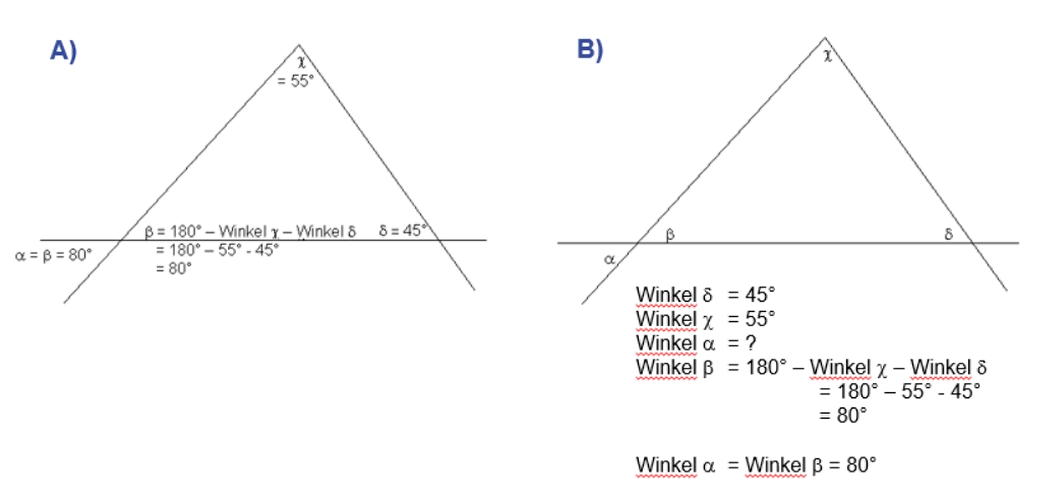
\includegraphics[width=\fpeval{0.7*\textwidth}pt]{Cognitive Load Theory.png}
    \begin{answers}
        \item[\correct] Abbildung A wird wahrscheinlich besser verarbeitet, da durch die räumliche Kontiguität die kognitive Belastung bei der Kohärenzbildung und somit die extrinsische Belastung minimiert wird.
        \item[\wrong] Abbildung A wird wahrscheinlich besser verarbeitet, da entsprechend dem Modalitätseffekt eine bessere Ausnutzung der Arbeitsgedächtniskapazität durch Belastung beider Subspeicher erreicht wird.
        \item[\wrong] Abbildung B wird wahrscheinlich besser verarbeitet, da es durch die Integration von aufeinander bezogenen Informationsquellen in Abbildung A zu einem Redundanzeffekt kommt. Die redundanten Informationen müssen ebenfalls verarbeitet werden und binden somit Arbeitsgedächtniskapazität.
        \item[\wrong] Abbildung B wird wahrscheinlich besser verarbeitet, da durch die Integration von aufeinander bezogenen Informationsquellen in Abbildung A eine Aufteilung der Aufmerksamkeit (split attention) befördert wird.
    \end{answers}
\end{multiple-choice}

\begin{multiple-choice}{Angebots-Nutzungsmodell}
    \assignment{Bitte kreuzen Sie die beiden richtigen Aussagen an!}
    \questiontext{In Hinblick auf das Angebots-Nutzungsmodell gilt:}
    \begin{answers}
        \item[\correct] Den Merkmalen der Schule kommt im Vergleich zu Merkmalen des Unterrichts eine geringere Bedeutung für dien Entwicklung der Lernenden zu.
        \item[\correct] Schulerfolg umfasst die Lern- und Leistungsentwicklung, die affektiv- motivationale sowie die persönlichkeitsbezogene Entwicklung der Lernenden.
        \item[\wrong] Mit Blick auf motivationale und persönlichkeitsbezogene Aspekte der Lehrperson geht man heute von direkten Effekten der beruflichen Motivation, der Persönlichkeit, des Belastungserlebens und der beruflichen Zufriedenheit auf den Schulerfolg der Lernenden aus.
        \item[\wrong] In Abhängigkeit von den individuellen Vorraussetzungen beeinflusst die mittlere Leistungsfähigkeit einer Klasse die Leistungsentwicklung eine*r Lernenden.
    \end{answers}
\end{multiple-choice}

\begin{mapping}{Erklärungsarten}
    \assignment{Ordnen Sie die Erklärungsarten dem jeweils passenden Beispiel zu.}
    \begin{answer}
        Pheromone werden von manchen Schmetterlingen gebildet, da sich die Geschlechtspartner über weite Entfernungen hinweg finden müssen. Demnach dienen Pheromone dem Zueinanderfinden der Geschlechtspartner bei Schmetterlingen.
        \ismappedto
        Kausalerklärung
    \end{answer}
    \begin{answer}
        Der Pudel (französisch Caniche) ist eine von der FCI anerkannte Hunderasse (FCI-Gruppe 9, Sektion 2, Standard Nr. 172). Pudel sind lebhaft und haben eine wollige, gekräuselte Behaarung. Pudel werden anhand ihrer Größe unterschiedlich benannt: Großpudel (auch Königspudel), Kleinpudel, Zwerggpudel und Toy-Pudel.
        \ismappedto
        Begriffserklärung
    \end{answer}
    \begin{answer}
        Das Sonnenlicht landet nicht direkt auf der Erdoberfläche. Es muss zunächst die Atmosphäre durchqueren. Auf dem Weg zur Erde trifft das Licht auf die verschiedensten Teilchen: Staub, Wassertröpfchen, die in der Luft schweben usw. Das Licht wird an diesen Teilchen umgeleitet, quasi in verschiedene Strahlen zerlegt. Diesen Vorgang bezeichnet man als Lichtstreuung. Die Stärke der Streuung des Lichts hängt von seiner Wellenlänge ab. Blaues Licht ist kurzwelliger als beispielsweise rotes Licht. Daher wird das blaue Licht stärker gestreut als das rote - der Himmel sieht blau aus.
        \ismappedto
        Funktionale Erklärung
    \end{answer}
    \begin{answer}
        Um die Fläche eine Dreiecks herauszufinden, multipliziere die Grundseite mal die Höhe und teile diese durch 2. So lautet die Flächen-Formel eines Dreiecks A = ½ gh.
    \end{answer}
    \begin{answer}
        Um die Fläche eines Dreiecks herauszufinden multiplizieredie Grundseite mal die Höhe und teile diese durch 2. Man dividiert durch 2 weil ein Parallelogramm in zwei Dreiecke geteilt werden kann. Da die Flächen-Formel eines Parallelogramm A = gh lautet, muss die Fläche eines Dreiecks die Hälfte eines Parallelogramms darstellen. So lautet die Flächen-Formel eines Dreiecks A = ½ gh.
    \end{answer}
\end{mapping}

\begin{mapping}{Maßnahmen zur Störungsprävention und -intervention}
    \questiontext{In Anlehnung an Fink und Halpern(2007) sowie Schnitzlbaumer (2010) wird bei Störungsprävention und -intervention ein schrittweises Verfahren empfohlen: 1. Primären Handlungsvektor stärken --> 2. Primären Handlungsvektor schützen --> 3. Konkurrierenden Handlungsvektor schwächen --> 4. Konkurrierenden Handlungsvektor beenden. Unten finden Sie verschiedene Präventions- und Interventionsmaßnahmen einer Lehrkraft. Ordnen Sie die vier genannten Schritte der jeweils passenden Maßnahmen zu.}
    \begin{answer}
        Die Lehrkraft lobt die mitarbeitenden Schüler*innen für ihr Engagement.
        \ismappedto
        Primären Handlungsvektor stärken
    \end{answer}
    \begin{answer}
        Die Lehrkraft ändert die Sitzordnung und setzt den*die störende*n Schüler*in um.
        \ismappedto
        Primären Handlungsvektor schützen
    \end{answer}
    \begin{answer}
        Die Lehrkraft bewegt sich in die Richtung des*der störenden Schüler*in und schüttelt den Kopf.
        \ismappedto
        Konkurrierenden Handlungsvektor schwächen
    \end{answer}
    \begin{answer}
        Die Lehrkraft hält kurz inne und nennt den Namen des*der störenden Schüler*in.
        \ismappedto
        Konkurrierenden Handlungsvektor beenden.
    \end{answer}
\end{mapping}

\begin{single-choice}{Instruktionale Erklärungen II}
    \assignment{Trifft folgende Aussage zu?\\„Expert Blind Spot“ beschreibt das Phänomen, dass Experten dazu neigen, dass Vorwissen von Novizen zu unterschätzen.}
    \begin{answers}
        \item[\correct] trifft nicht zu
        \item[\wrong] trifft zu
    \end{answers}
\end{single-choice}

\begin{multiple-choice}{Kooperatives Lernen I}
    \assignment{Bitte kreuzen Sie die richtige(n) Aussage(n) an!}
    \questiontext{In Bezug auf kooperatives Lernen gilt:}
    \begin{answers}
        \item[\correct] Individuelle Verantwortlichkeit gehört nicht zu den Basismerkmalen nach Johnson \& Johnson (1986).
        \item[\correct] Zu den Lesestrategien beim Reciprocal Teaching zählen das Fragen stellen, Zusammenfassungen geben, das Klären unklarer Textabschnitte sowie das Treffen von Vorhersagen.
        \item[\wrong] Das Basismerkmal der \textit{positiven Interdependenz} wirkt den Phänomenen „Der Hans macht es doch eh“ und „Ja bin ich denn der Depp“ nicht entgegen.
        \item[\wrong] Individuelle Verantwortlichkeit ist ein Basismerkmal, welches bei der Gruppenrallye (auch Student Team Achievement Divisions, kurz: STAD, genannt) zum Tragen kommt.
    \end{answers}
\end{multiple-choice}


\end{document}